\documentclass[a4paper,fleqn]{tufte-handout} 
\usepackage{graphicx}

\title{Computational experiments in Science : herding horses on a daily basis}

\author{Mathieu Lagrange}

\begin{document}

\maketitle

\section{Introduction}

Dealing with large amount of numerical data and complex processes is the chance or the curse of a lot of fields in science. Contrary to pure engineering approaches where the main objective is the performance, the main of science is, by experimental demonstration, to confirm or reject reasonable assumptions that have been formulated theoretically. That being said, those two approaches have in common the need to perform some kind of experiment which in most cases resort to 1) take data from measurements, 2) process it using algorithms built upon some assumptions about the underlying process that generated the data, 3) study if those algorithms are able to produce corresponding data that, in the engineering scenario, tentatively serves some useful purpose and in the science one, potentially validates the theory.


\section{Horses are where complexity is}

Data under evaluation in today(s challenges, are highly multidimensional in many ways, number of dimensions, number of items, number of classes. Fully understanding the complexity behind this is an utopia rather than an achievable goal and as such every conclusion that are drawn are to be considered with care.

An issue that arises is the fact that, even if the underlying assumption that helped us to build a processing chain is correct, the implemented machine is in fact using other means to achieve the good results we are striving for. More precisely, a "horse" is a system appearing capable of a remarkable human feat, e.g., music genre recognition from an audio signal, but actually working by using irrelevant characteristics (confounds) \citep{6847693}.

Adopting a purely engineering approach, leaves us with the freedom to live with horses without to much concerns as only the end performance counts. On contrary, science is not supposed to "ride" horses as engineering approaches can as it may lead to an erroneous validation of a given theory or assumption.

\section{Spotting a horse}

\cite{aucouturier2007bag}

\cite{lagrange:hal-01082501}

\section{Herding horses}



\subsection{Data}

\begin{marginfigure}
\begin{center}
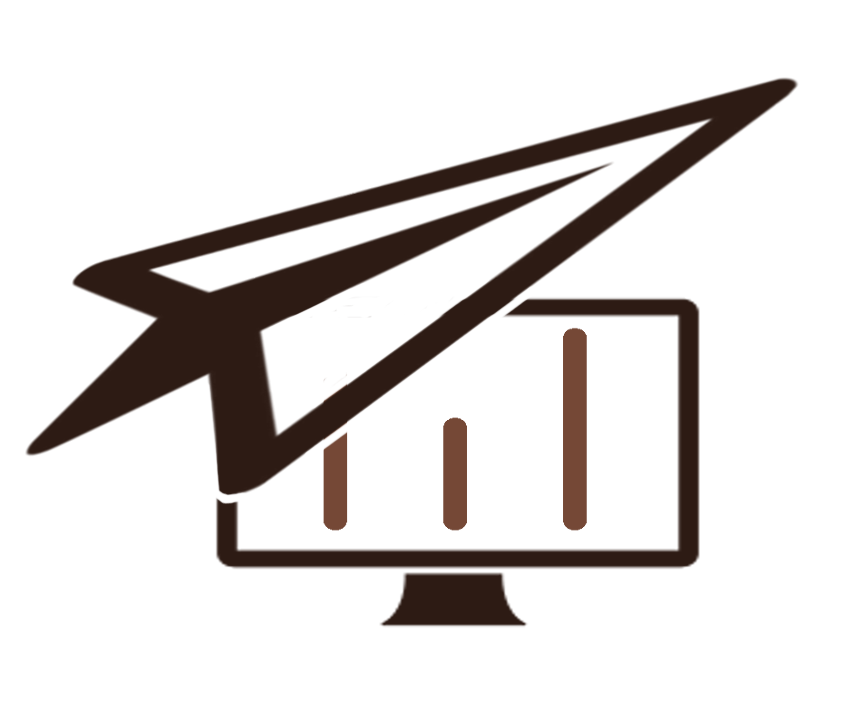
\includegraphics[width=\textwidth]{figures/logo} 
\end{center}
\caption{\label{fig:simScene} SimScene is an open source tool: \url{https://bitbucket.org/mlagrange/simscene}}
\end{marginfigure}

\begin{enumerate}
\item carefully craft evaluation datasets (big is not enough)
\item increase the complexity progressively with controled simulated data
\end{enumerate}



\subsection{Experimentation}

\begin{marginfigure}
\begin{center}
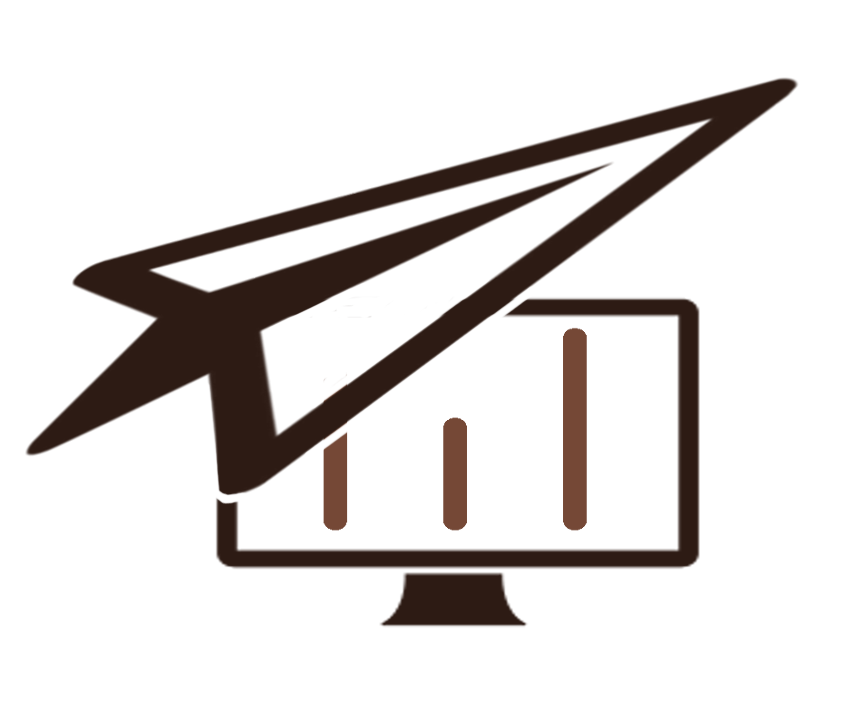
\includegraphics[width=\textwidth]{figures/logo} 
\end{center}
\caption{\label{fig:explanes} ExpLanes is an open source tool: \url{http://mathieulagrange.github.io/expLanes}}
\end{marginfigure}

\begin{enumerate}
\item implement lower bound and upper bounds baselines
\item enforce reproducibility
\end{enumerate}




  
\bibliographystyle{abbrvnat} 
\bibliography{bib} 
  
\end{document}